%%%%%%%%%%%%%%%%%%%%%%%%%%%%%%%%%%%%%%%%%
% Beamer Presentation
% LaTeX Template
% Version 1.0 (10/11/12)
%
% This template has been downloaded from:
% http://www.LaTeXTemplates.com
%
% License:
% CC BY-NC-SA 3.0 (http://creativecommons.org/licenses/by-nc-sa/3.0/)
%
%%%%%%%%%%%%%%%%%%%%%%%%%%%%%%%%%%%%%%%%%

%----------------------------------------------------------------------------------------
%	PACKAGES AND THEMES
%----------------------------------------------------------------------------------------

\documentclass{beamer}

\mode<presentation> {

% The Beamer class comes with a number of default slide themes
% which change the colors and layouts of slides. Below this is a list
% of all the themes, uncomment each in turn to see what they look like.

%\usetheme{default}
%\usetheme{AnnArbor}
%\usetheme{Antibes}
%\usetheme{Bergen}
%\usetheme{Berkeley}
%\usetheme{Berlin}
%\usetheme{Boadilla}
%\usetheme{CambridgeUS}
%\usetheme{Copenhagen}
%\usetheme{Darmstadt}
%\usetheme{Dresden}
%\usetheme{Frankfurt}
%\usetheme{Goettingen}
%\usetheme{Hannover}
%\usetheme{Ilmenau}
%\usetheme{JuanLesPins}
%\usetheme{Luebeck}
%\usetheme{Madrid}
\usetheme[sectionpage=progressbar, progressbar=frametitle, numbering=fraction]{metropolis}
%\usetheme{Malmoe}
%\usetheme{Marburg}
%\usetheme{Montpellier}
%\usetheme{PaloAlto}
%\usetheme{Pittsburgh}
%\usetheme{Rochester}
%\usetheme{Singapore}
%\usetheme{Szeged}
%\usetheme{Warsaw}

% As well as themes, the Beamer class has a number of color themes
% for any slide theme. Uncomment each of these in turn to see how it
% changes the colors of your current slide theme.

%\usecolortheme{albatross}
%\usecolortheme{beaver}
%\usecolortheme{beetle}
%\usecolortheme{crane}
%\usecolortheme{dolphin}
%\usecolortheme{dove}
%\usecolortheme{fly}
%\usecolortheme{lily}
%\usecolortheme{orchid}
%\usecolortheme{rose}
%\usecolortheme{seagull}
%\usecolortheme{seahorse}
%\usecolortheme{whale}
%\usecolortheme{wolverine}

%\setbeamertemplate{footline} % To remove the footer line in all slides uncomment this line
%\setbeamertemplate{footline}[page number] % To replace the footer line in all slides with a simple slide count uncomment this line

%\setbeamertemplate{navigation symbols}{} % To remove the navigation symbols from the bottom of all slides uncomment this line

}

% http://www-ljk.imag.fr/membres/Jerome.Lelong/latex/appendixnumberbeamer.sty
% Reference: http://tex.stackexchange.com/questions/2541/beamer-frame-numbering-in-appendix
\usepackage{appendixnumberbeamer}
% Add total frame count to slides, optional. From Stefan,
% http://www.latex-community.org/forum/viewtopic.php?f=4&t=2173
\expandafter\def\expandafter\insertshorttitle\expandafter{%
  \insertshorttitle\hfill\insertframenumber\,/\,\inserttotalframenumber}

\makeatletter
\newcommand{\srcsize}{\@setfontsize{\srcsize}{5pt}{5pt}}
\makeatother

\usepackage{mathtools}
\usepackage{tabularx}

\usepackage[english]{babel}
\usepackage[utf8]{inputenc}

\newcommand{\backupbegin}{
   \newcounter{finalframe}
   \setcounter{finalframe}{\value{framenumber}}
}
\newcommand{\backupend}{
   \setcounter{framenumber}{\value{finalframe}}
}

\usepackage{soul} % use this (many fancier options)

\usepackage{listings}
\lstset{
  language=JAVA,
  captionpos=b,
  escapeinside={(*@}{@*)}, 
  breaklines=true
}

\newcommand{\rot}[1]{\rotatebox{#1}}
\usepackage{tabularx}

\usepackage{algorithm}
\usepackage{algorithmic}
\renewcommand{\algorithmicrequire}{\textbf{Input:}}
\renewcommand{\algorithmicensure}{\textbf{Output:}}


\definecolor{ForestGreen}{rgb}{0.13,0.54,0.13}

\usepackage{adjustbox}

\usepackage{graphicx} % Allows including images
\usepackage{booktabs} % Allows the use of \toprule, \midrule and \bottomrule in tables

%----------------------------------------------------------------------------------------
%	TITLE PAGE
%----------------------------------------------------------------------------------------

\title[Spoon: a multi-tool Java library for Java]{Spoon: Open Source Library to Analyze, Rewrite, Transform, Transpile Java Source Code - A getting started} % The short title appears at the bottom of every slide, the full title is only on the title page

\author{Simon Urli \\ \url{simon.urli@inria.fr} \\\texttt{https://github.com/INRIA/spoon}} % Your name
\institute[Inria \& University of Lille] % Your institution as it will appear on the bottom of every slide, may be shorthand to save space
{
\medskip
\textit{OW2Con'18}\\ % Your email address
\medskip
\vspace{px}
}
\date{7th, June 2018} % Date, can be changed to a custom date

\titlegraphic{
\vspace{200px}

\includegraphics[width=50px]{figures/title/logos/inria-logo.png}

\includegraphics[width=50px]{figures/title/logos/ow2.png}
}

\begin{document}

\begin{frame}
\maketitle
\end{frame}

\begin{frame}{History \& Community}
\begin{columns}
\begin{column}{0.5\textwidth}
\begin{itemize}
\item 2005: project creation at INRIA Lille
\item 2014: Spoon on Github
\item 2016: Spoon at OW2
\item 2017: Community Award at OW2Con
\end{itemize}
\end{column}
\begin{column}{0.6\textwidth}  %%<--- here
   \begin{center}
   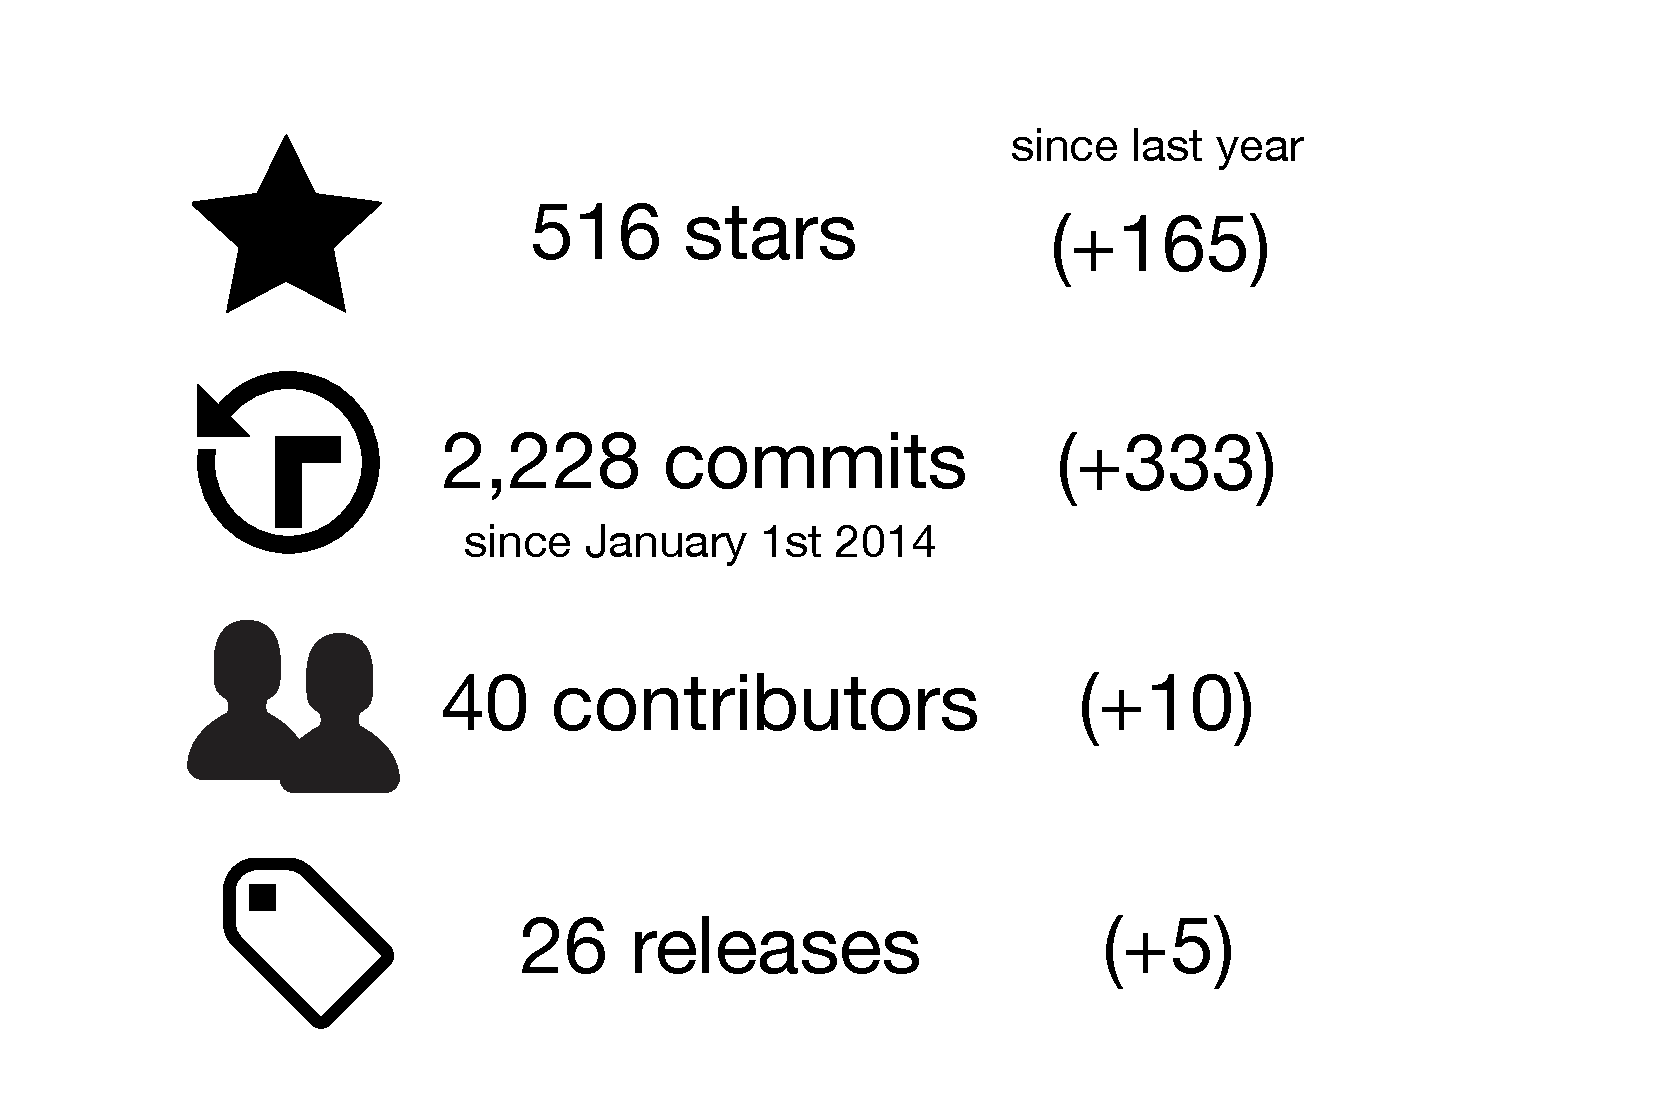
\includegraphics[width=\textwidth]{figures/title/stats.pdf}
   \end{center}
\end{column}
\end{columns}


\end{frame}

\begin{frame}{Spoon in a nutshell}
\centering
A library to write your own analysis and transformation in java.\\
\vspace{10px}
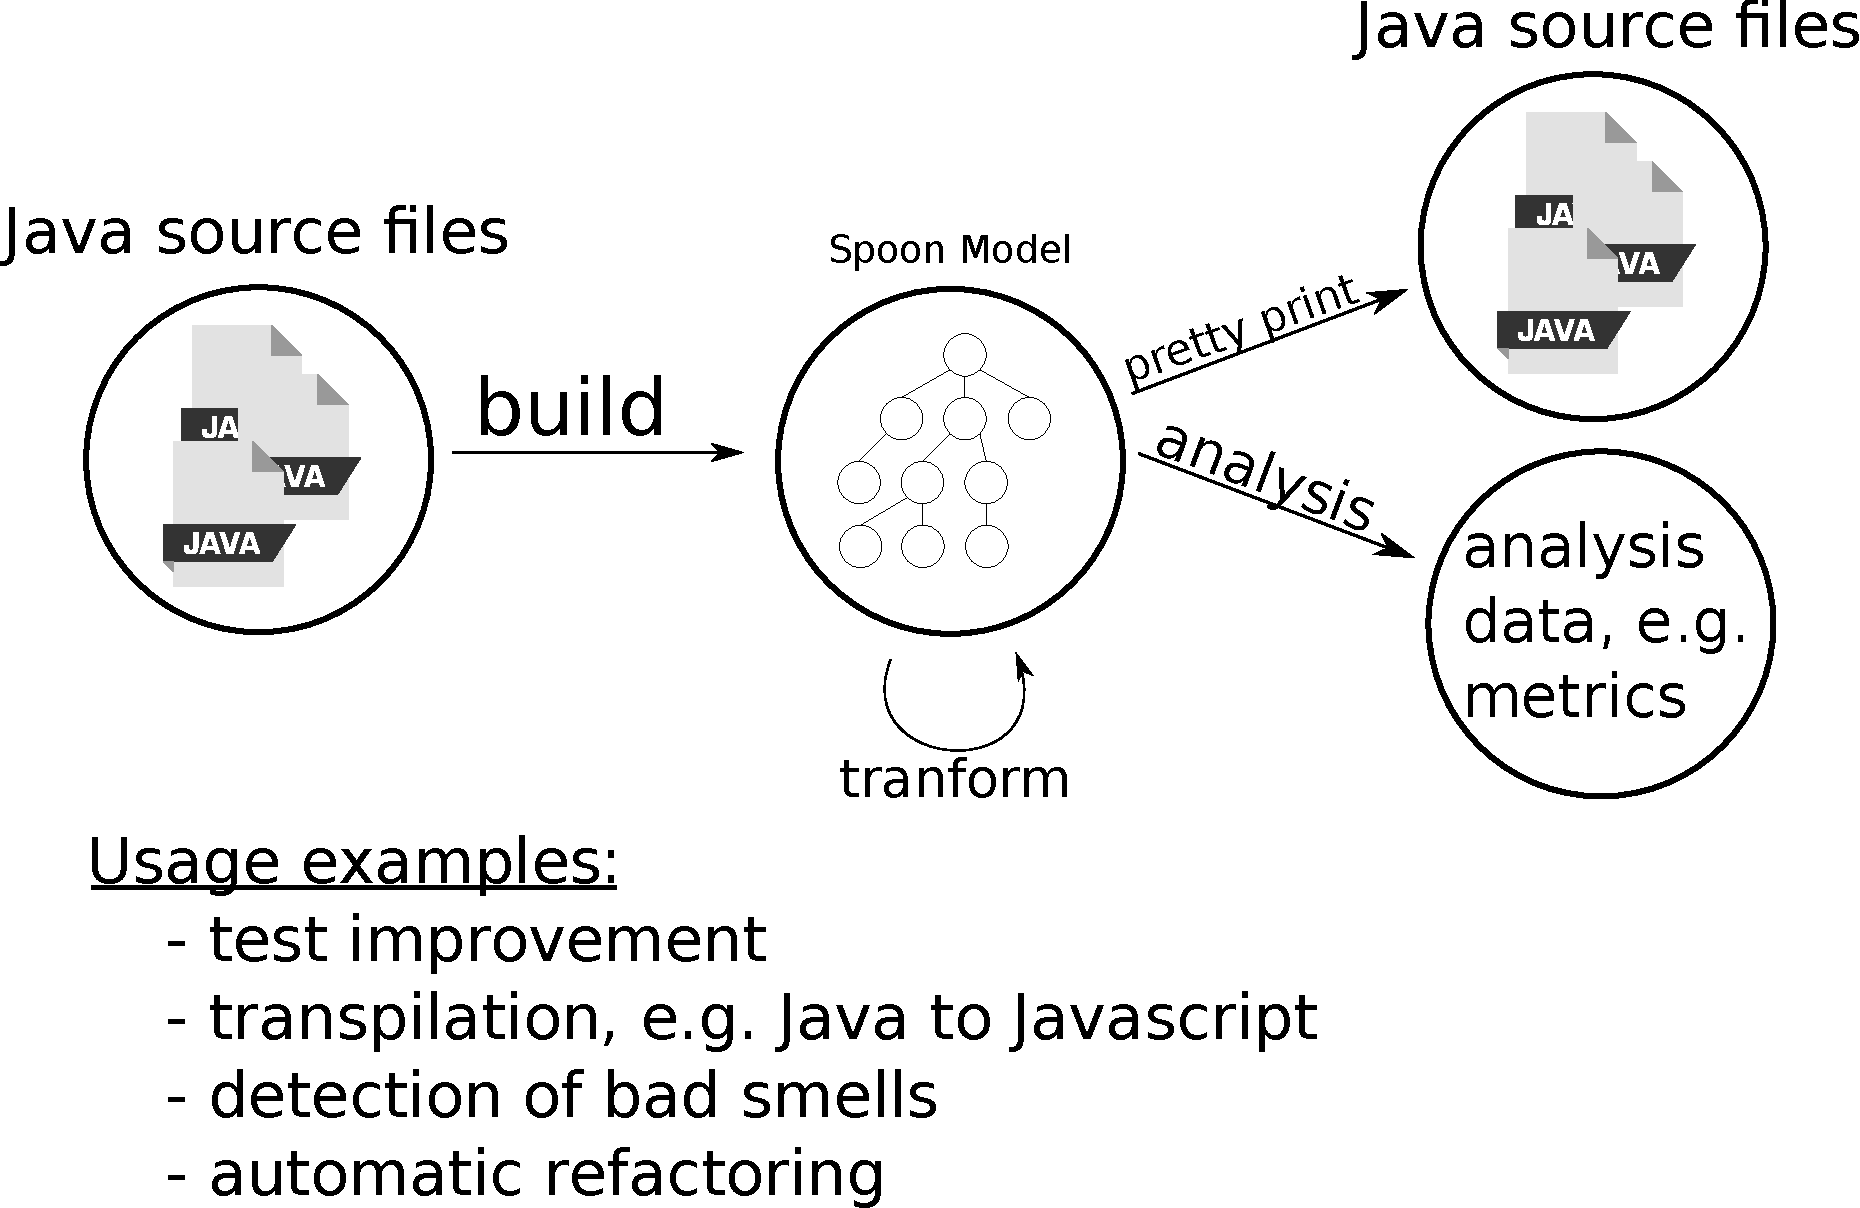
\includegraphics[scale=0.32]{figures/overview-1.pdf}
\end{frame}

% Change name to  funny in example. (no Example etc...)

%----------------------------------------------------------------------------------------
%	SPOON
%----------------------------------------------------------------------------------------

\section{Spoon Overview}

\begin{frame}{Spoon standard process}

\begin{enumerate}
\item Build a model of your project
\item Query and analyze interesting parts
\item Transform what needs to be transformed
\item Output a transformed source code
\end{enumerate}

\end{frame}

\begin{frame}{Building a Spoon model}

Inputs:
\begin{itemize}
\item Source code (i.e. java files or snippets)
\item Many options like classpath, Java version, ...
\end{itemize}

Output:
\begin{itemize}
\item Spoon model
\end{itemize}
\end{frame}

\begin{frame}{Spoon AST Metamodel (excerpt)}
\begin{figure}
\centering
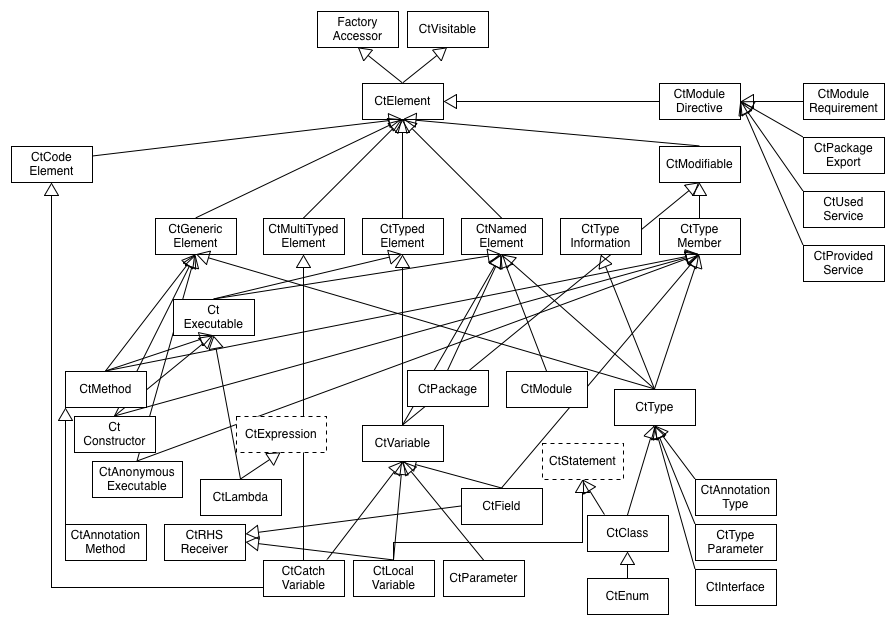
\includegraphics[width=\textwidth]{figures/model/structural-elements.png}
\end{figure}
\end{frame}

\begin{frame}{Spoon model example}
\begin{figure}
\centering
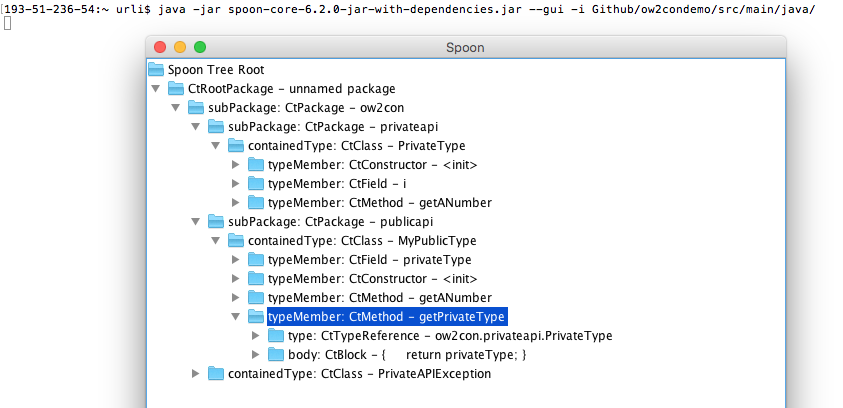
\includegraphics[width=\textwidth]{figures/model/spoon-model.png}
\end{figure}
\end{frame}

\begin{frame}{Query and analyze model}
Different ways of doing it:
\begin{itemize}
\item Using Query API (filter-chaining API)
\item Using XPath-like API
\end{itemize}
\end{frame}

\begin{frame}{Transform model}
Transforming model involve performing basic CRUD operations on the nodes of the model.

\end{frame}

\begin{frame}{Transform model}
Transforming model involve performing basic CRUD operations on the nodes of the model.
\begin{itemize}
\item Create a node
\end{itemize}

\begin{figure}
\centering
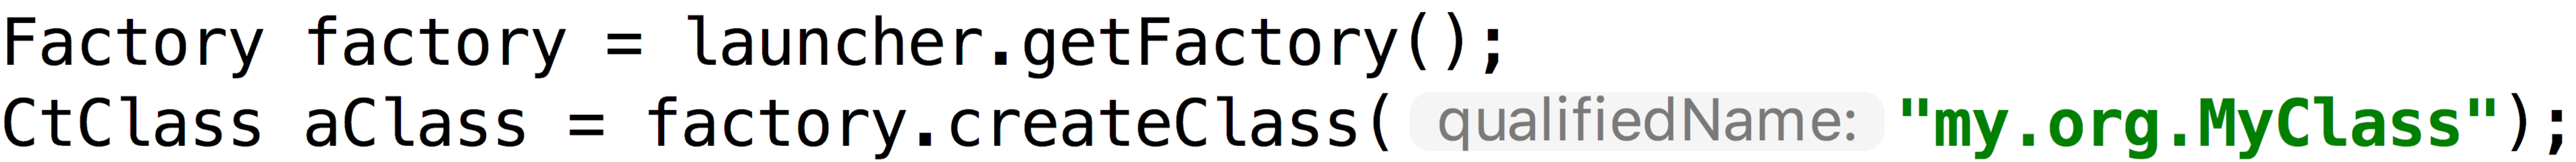
\includegraphics[width=\textwidth]{figures/transform/transfo-add}
\end{figure}
\end{frame}

\begin{frame}{Transform model}

Transforming model involve performing basic CRUD operations on the nodes of the model.
\begin{itemize}
\item Create a node
\item Update a node
\end{itemize}

\begin{figure}
\centering
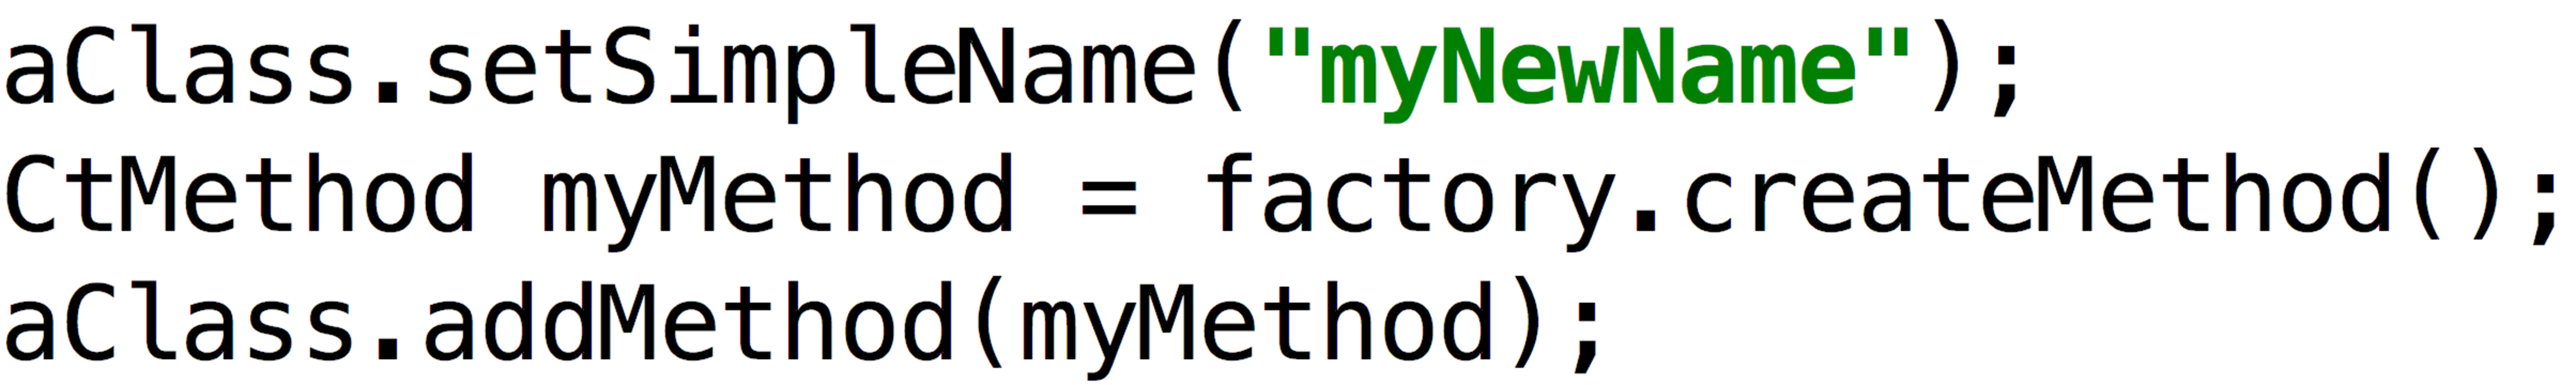
\includegraphics[width=\textwidth]{figures/transform/transfo-update.pdf}
\end{figure}
\end{frame}

\begin{frame}{Transform model}

Transforming model involve performing basic CRUD operations on the nodes of the model.
\begin{itemize}
\item Create a node
\item Update a node
\item Delete a node
\end{itemize}

\begin{figure}
\centering
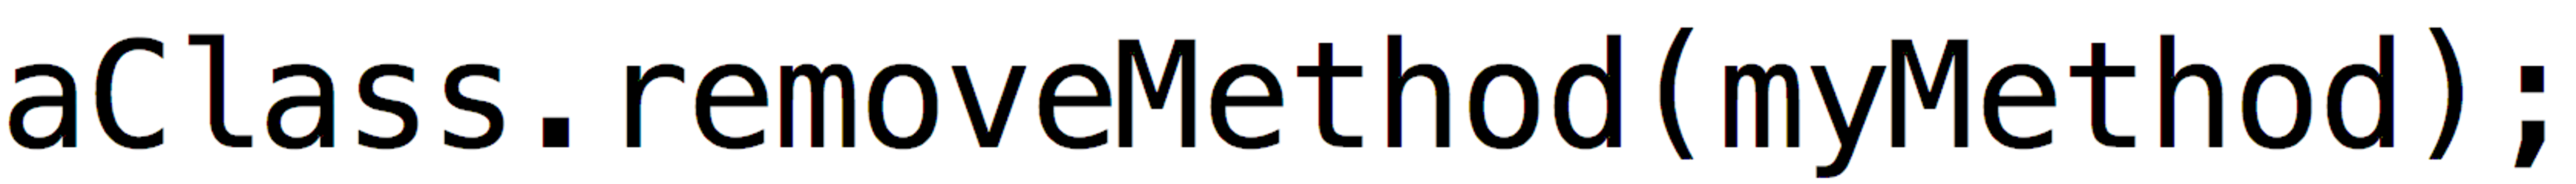
\includegraphics[width=\textwidth]{figures/transform/transfo-delete.pdf}
\end{figure}
\end{frame}

\begin{frame}{Output the model}
Spoon provides a default Java pretty-printer:
\begin{itemize}
\item output the model using standard Java code-style
\item create files hierarchy based on the compilation units or types
\end{itemize} 
\end{frame}

\section{Quick scenario}

\begin{frame}{Scenario}

You want to enforce that all types from the \textbf{private API} are not returned from the \textbf{public API}.

\begin{figure}
\centering
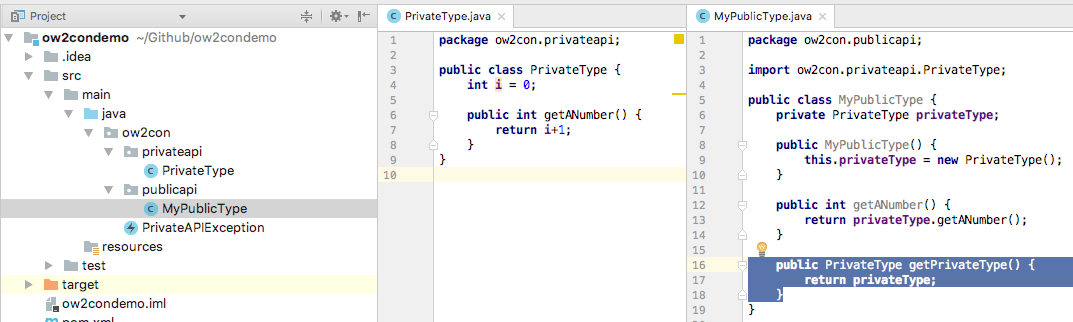
\includegraphics[width=\textwidth]{figures/scenario.png}
\end{figure}

\end{frame}

\section{Building the model}

\begin{frame}[t]{Building a Spoon model from Maven}

From a Maven Project:
\begin{figure}
\centering
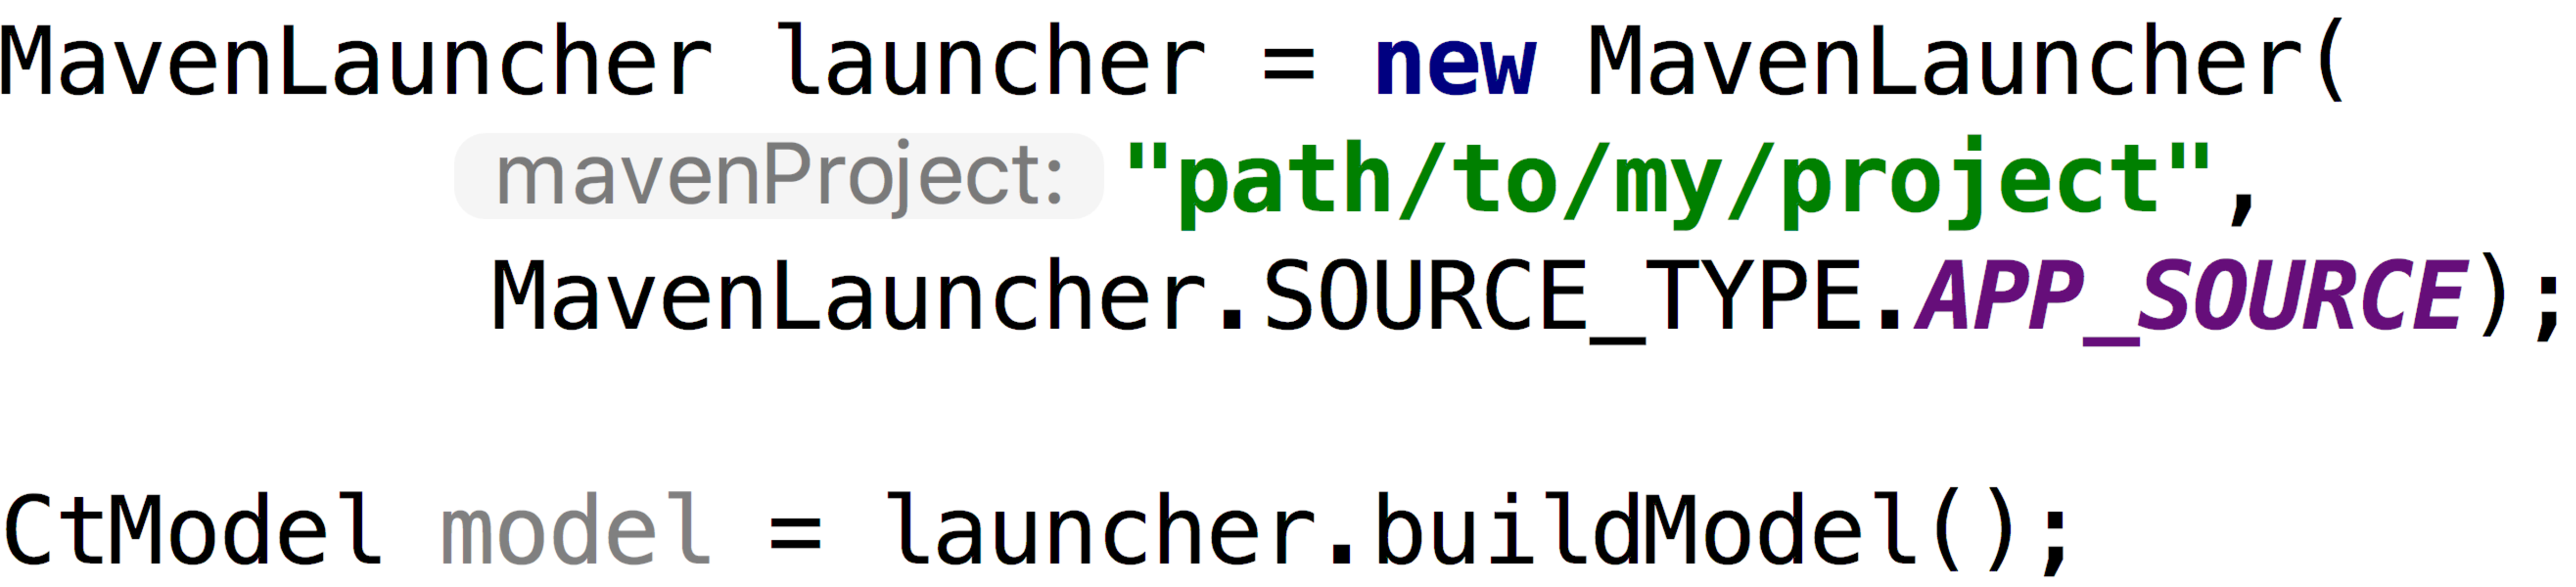
\includegraphics[width=0.8\textwidth]{figures/build/maven-launcher.pdf}
\end{figure}

Automatically get the libraries from Maven dependencies.
\end{frame}

\begin{frame}[t]{Building a Spoon model from sources}

From input source of a project:
\begin{figure}
\centering
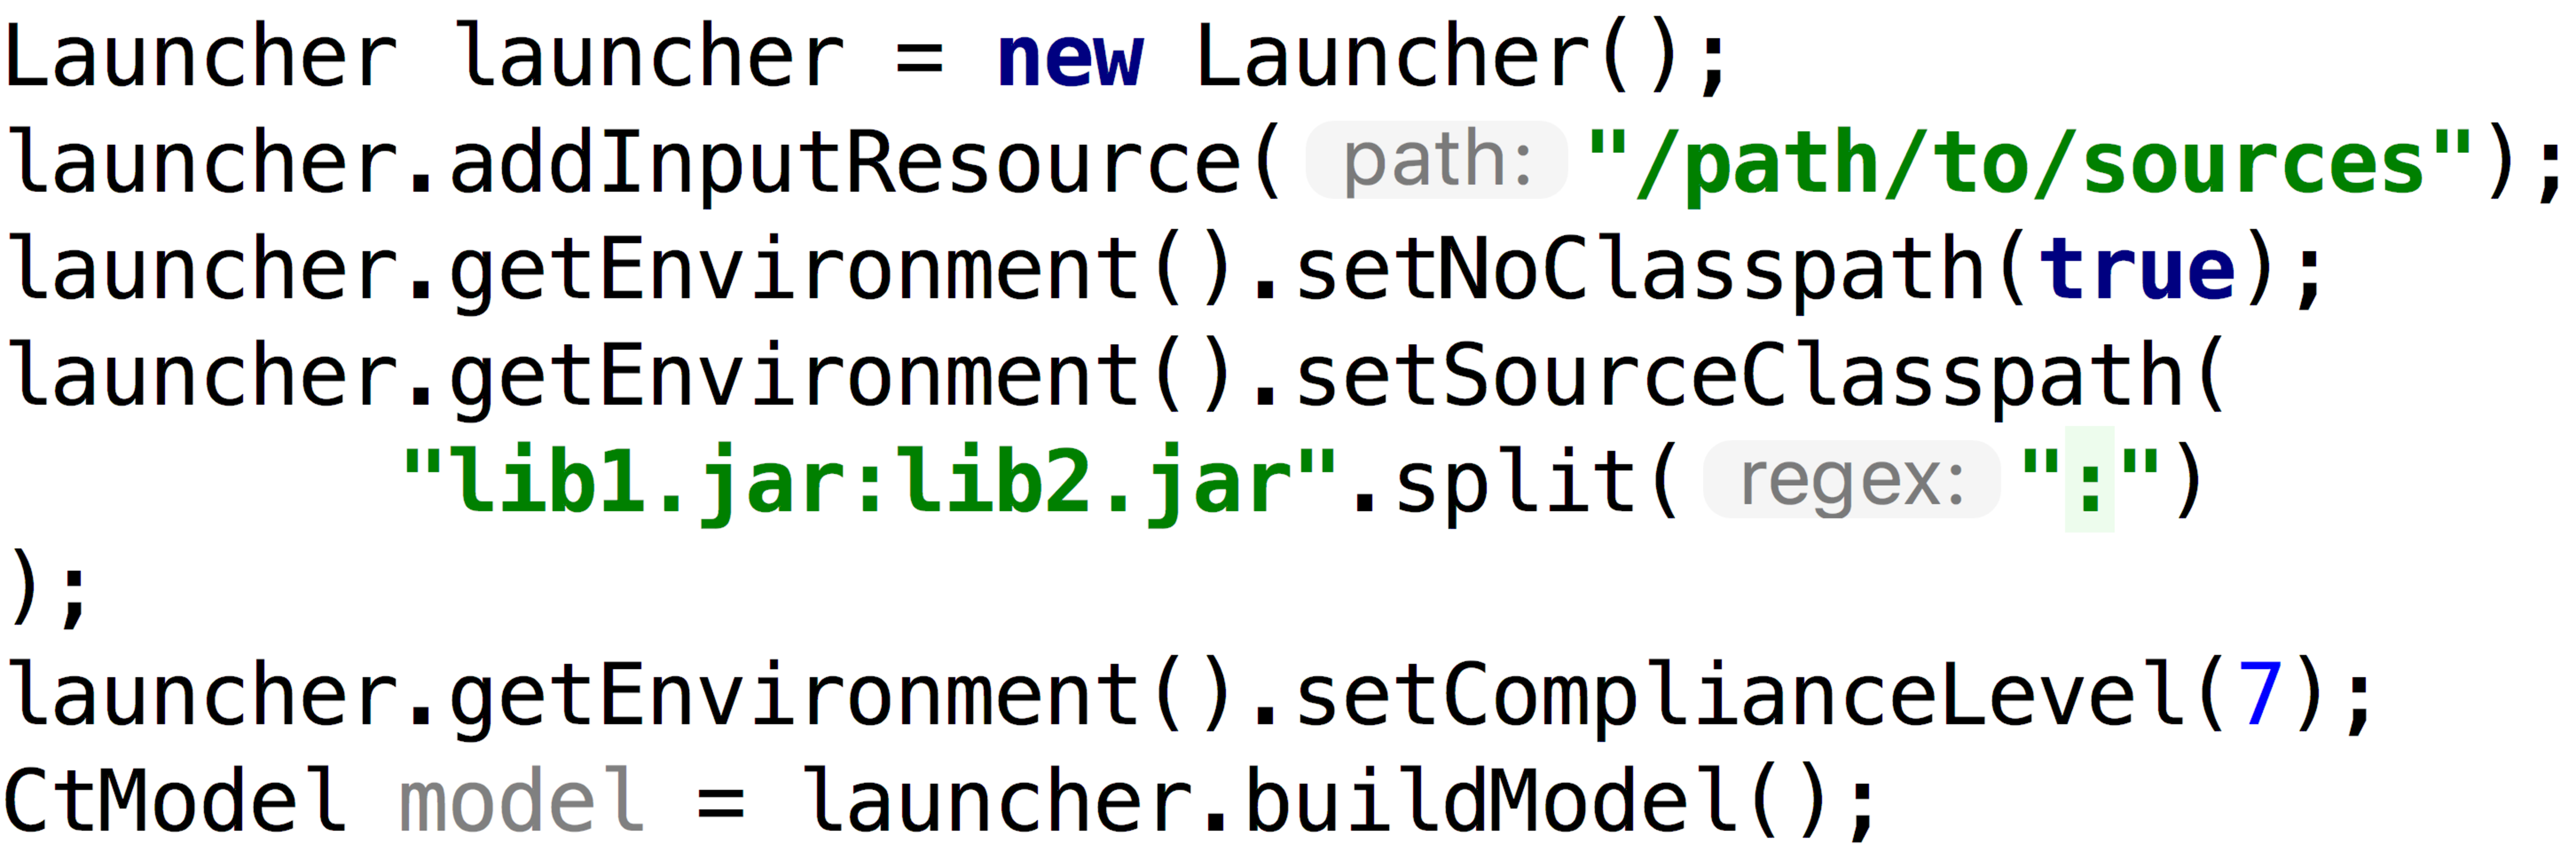
\includegraphics[width=\textwidth]{figures/build/api-launcher.pdf}
\end{figure}

Be careful with the classpath of your project. Don't hesitate to use \texttt{noclasspath} mode. (default in next version of Spoon)
\end{frame}

\begin{frame}[t]{Query and analyze model: scenario}

Goal: 
\begin{enumerate}
\item retrieve all types from the public API package
\end{enumerate}

\begin{figure}
\centering

\includegraphics[width=\textwidth]{figures/queries/query-scenario-1.pdf}
\end{figure}
\end{frame}

\begin{frame}[t]{Query and analyze model: scenario}

Goal:
\begin{enumerate}
\item retrieve all types from the public API package
\item retrieve all methods from those types
\end{enumerate}

\begin{figure}
\centering

\includegraphics[width=\textwidth]{figures/queries/query-scenario-2.pdf}
\end{figure}
\end{frame}

\begin{frame}[t]{Query and analyze model: scenario}

Goal:
\begin{enumerate}
\item retrieve all types from the public API package
\item retrieve all methods from those types
\item retrieve methods that are public
\end{enumerate}

\begin{figure}
\centering

\includegraphics[width=\textwidth]{figures/queries/query-scenario-3.pdf}
\end{figure}
\end{frame}

\begin{frame}[t]{Query and analyze model: scenario}
Goal:
\begin{enumerate}
\item retrieve all types from the public API package
\item retrieve all methods from those types
\item retrieve methods that are public 
\item and returns a type from the private API package
\end{enumerate}

\begin{figure}
\centering

\includegraphics[width=\textwidth]{figures/queries/query-scenario-4.pdf}
\end{figure}
\end{frame}

\begin{frame}{Transform model: scenario - Plan}
Goal: prevent using the detected methods

How to do it? 
\begin{itemize}
\item Comments all statements
\item Throw a dedicated RuntimeException
\item Add an explanatory comment
\end{itemize}

Remember: it's only an educational example :-)
\end{frame}

\begin{frame}[t]{Transform model: scenario - Which exception?}

What exception should be throw?

We actually already have one!
\begin{figure}
\centering
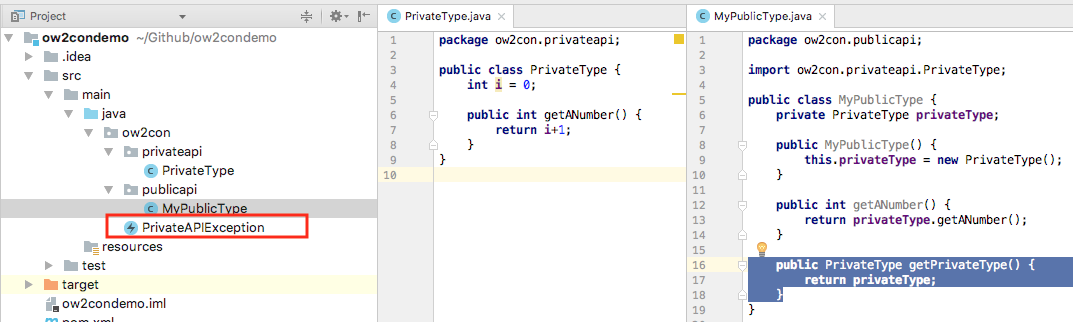
\includegraphics[width=\textwidth]{figures/scenario-exception.png}
\end{figure}
\end{frame}

\begin{frame}[t]{Transform model: hands on!}

Goal: Get the exception class.
\begin{figure}
\centering

\includegraphics[width=\textwidth]{figures/transform/transfo-scenario-1.pdf}
\end{figure}
\end{frame}

\begin{frame}[t]{Transform model: hands on!}

Goal: Create an instance of the exception class.
\begin{figure}
\centering

\includegraphics[width=\textwidth]{figures/transform/transfo-scenario-2.pdf}
\end{figure}
\end{frame}

\begin{frame}[t]{Transform model: hands on!}

Goal: Iterate over the queried methods.
\begin{figure}
\centering

\includegraphics[width=\textwidth]{figures/transform/transfo-scenario-3.pdf}
\end{figure}
\end{frame}

\begin{frame}[t]{Transform model: hands on!}

Goal: Create comments for all statements.
\begin{figure}
\centering
\includegraphics[width=\textwidth]{figures/transform/transfo-scenario-4.pdf}
\end{figure}
\end{frame}

\begin{frame}[t]{Transform model: hands on!}

Goal: Create a new \textbf{throw} statement with the call to the new instance of the exception. 
\begin{figure}
\centering
\includegraphics[width=\textwidth]{figures/transform/transfo-scenario-5.pdf}
\end{figure}
\end{frame}

\begin{frame}[t]{Transform model: hands on!}

Goal: Add a final explanatory comment.
\begin{figure}
\centering
\includegraphics[width=\textwidth]{figures/transform/transfo-scenario-6.pdf}
\end{figure}
\end{frame}

\begin{frame}[c]{Let's output the model}
\begin{figure}
\centering
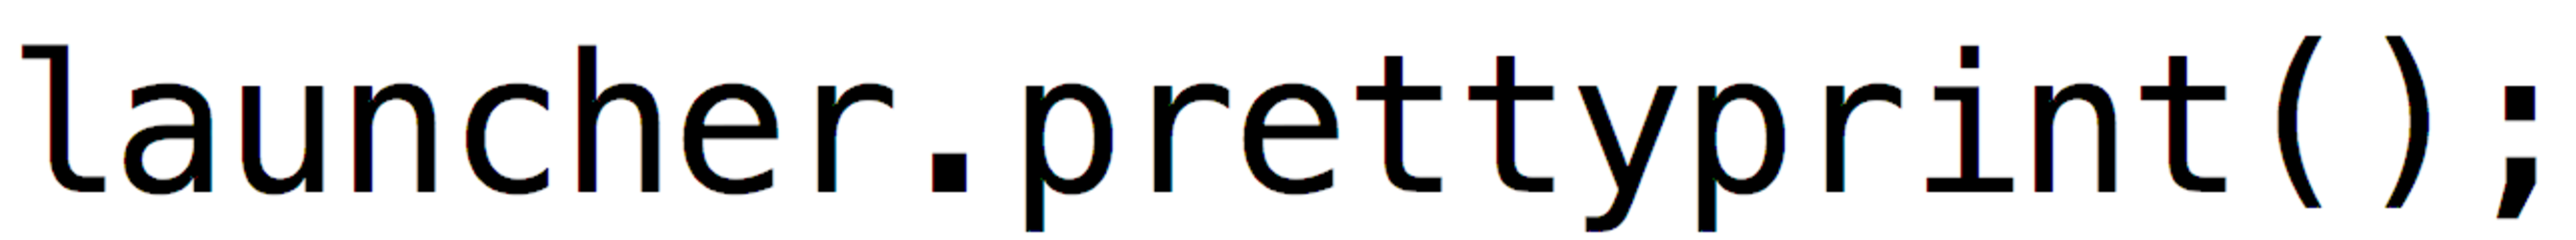
\includegraphics[width=\textwidth]{figures/output/pretty-print.pdf}
\end{figure}
\end{frame}

\begin{frame}[t]{Output the model: scenario}
What about the imports and comments?
\begin{figure}
\centering
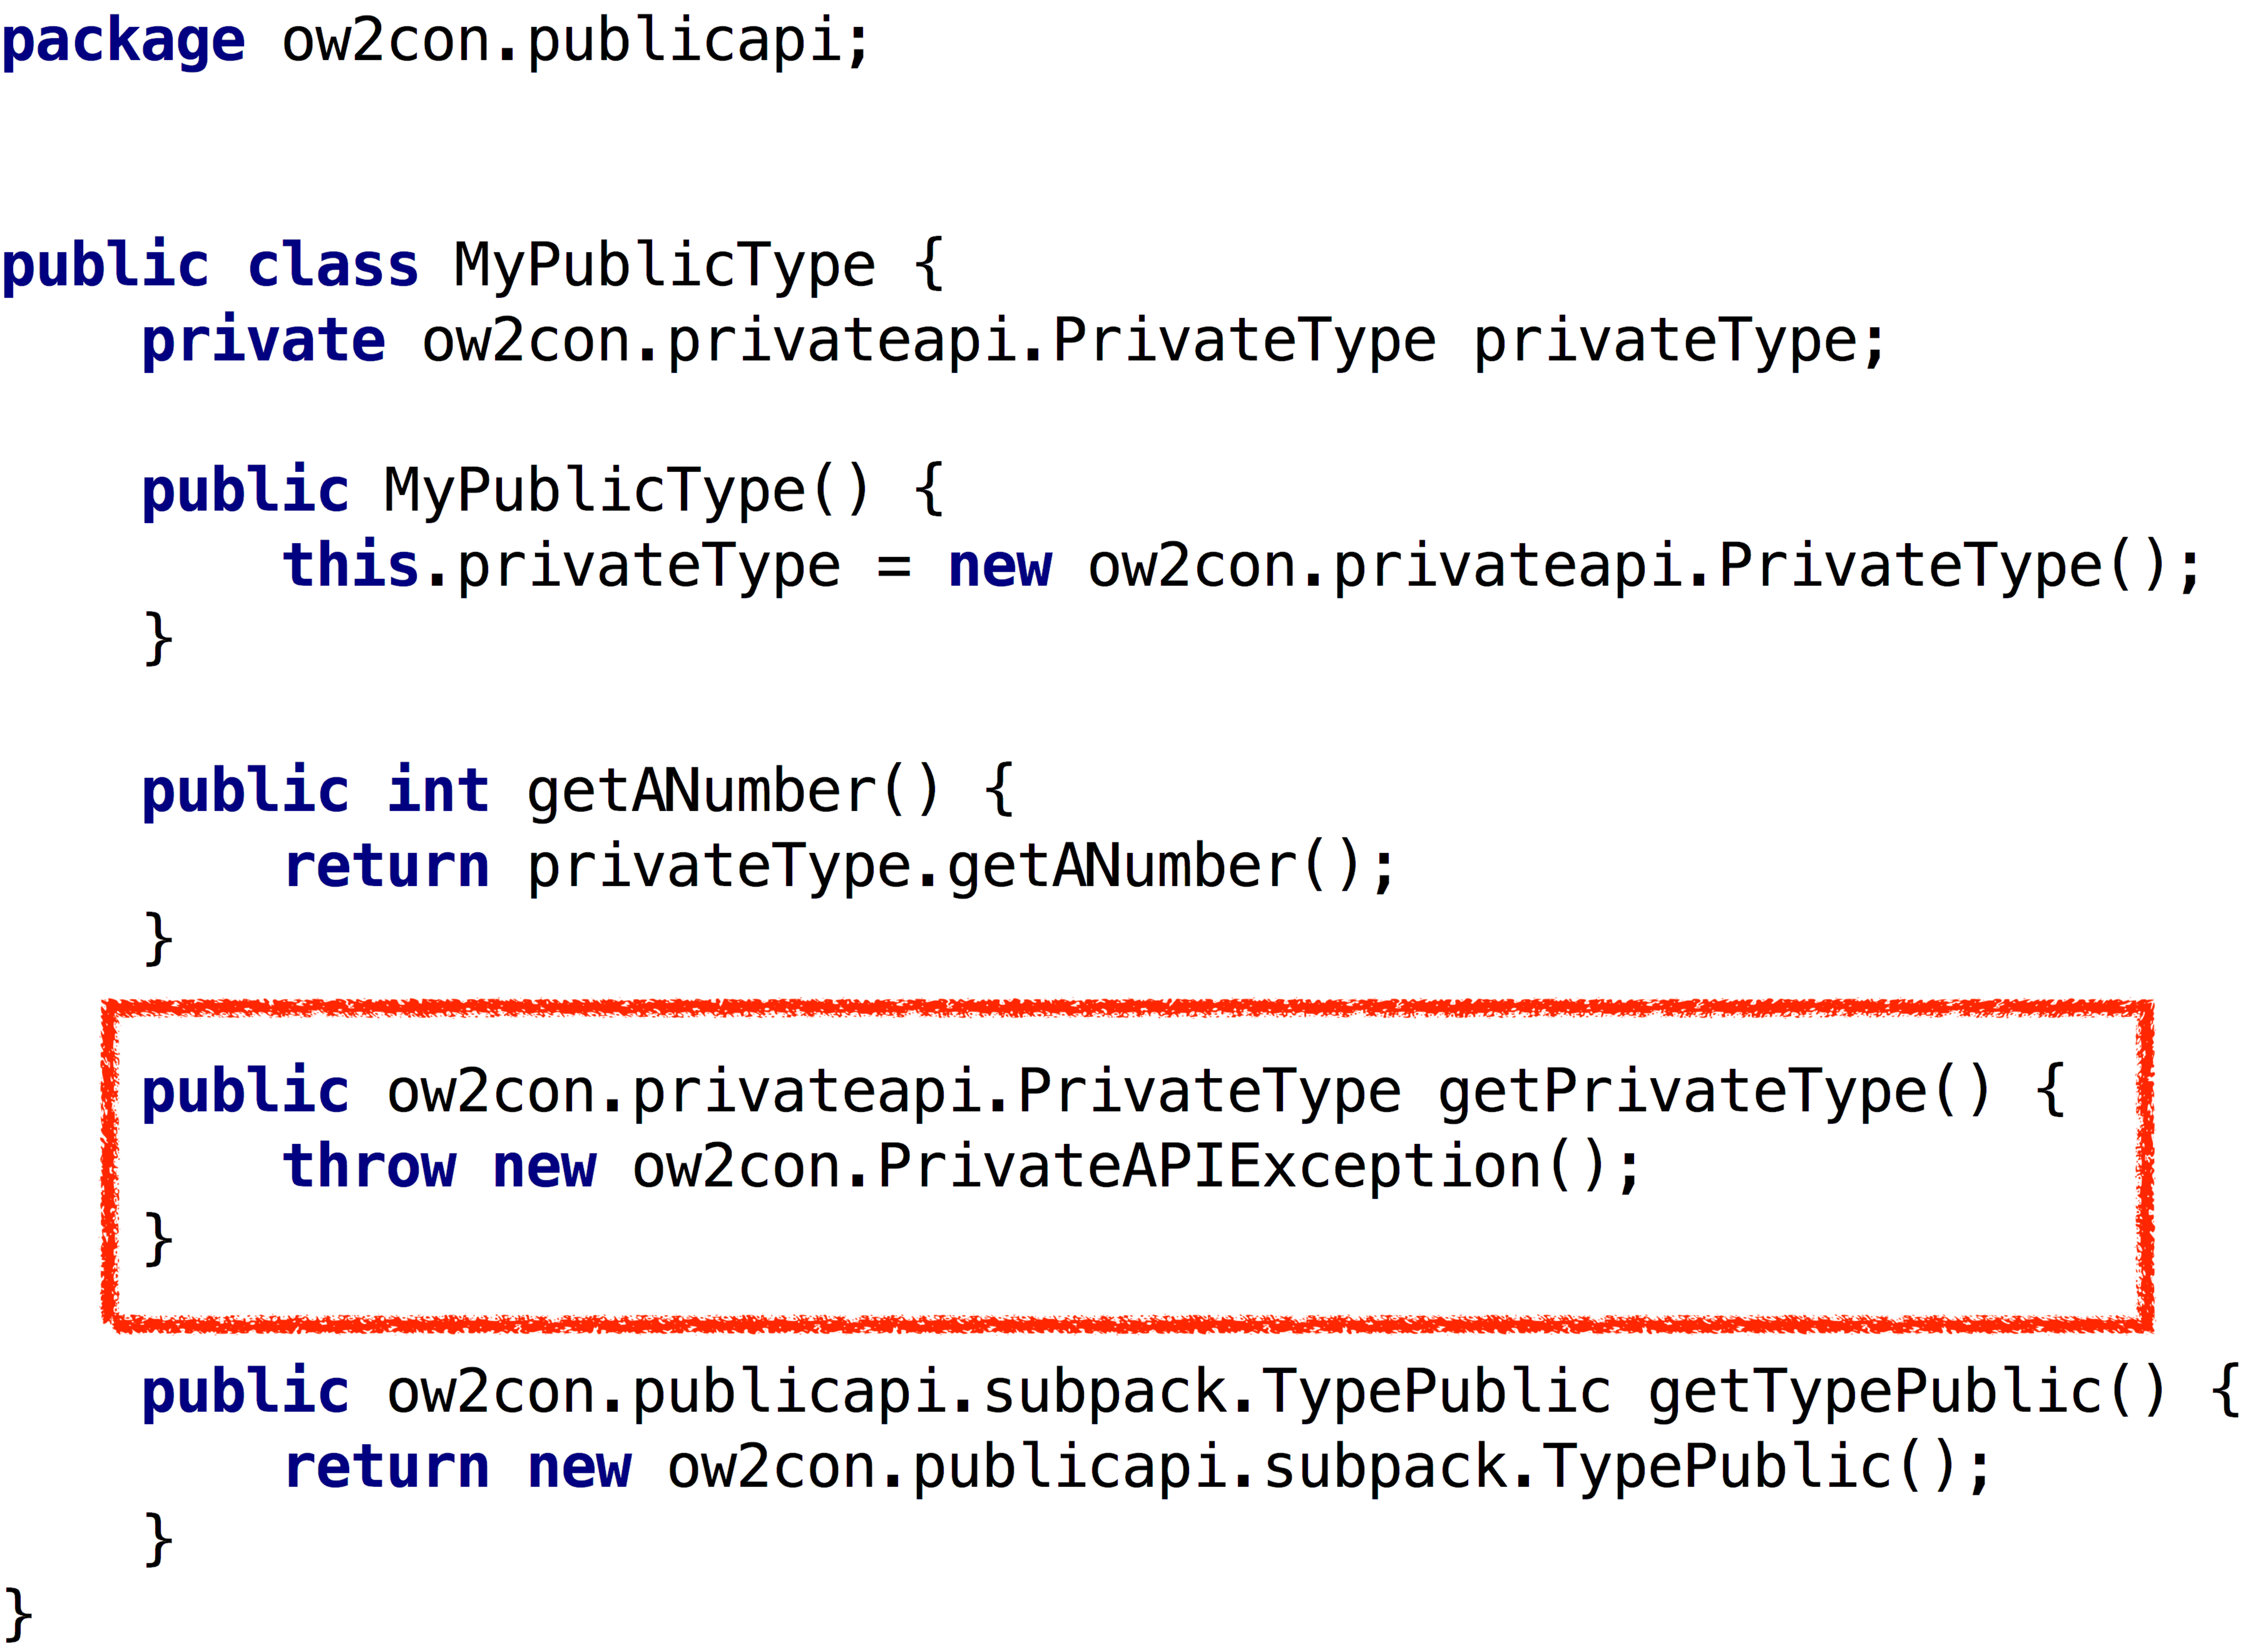
\includegraphics[width=\textwidth]{figures/output/scenario-result-1.pdf}
\end{figure}
\end{frame}

\begin{frame}{Manage imports and comments}

\begin{figure}
\centering
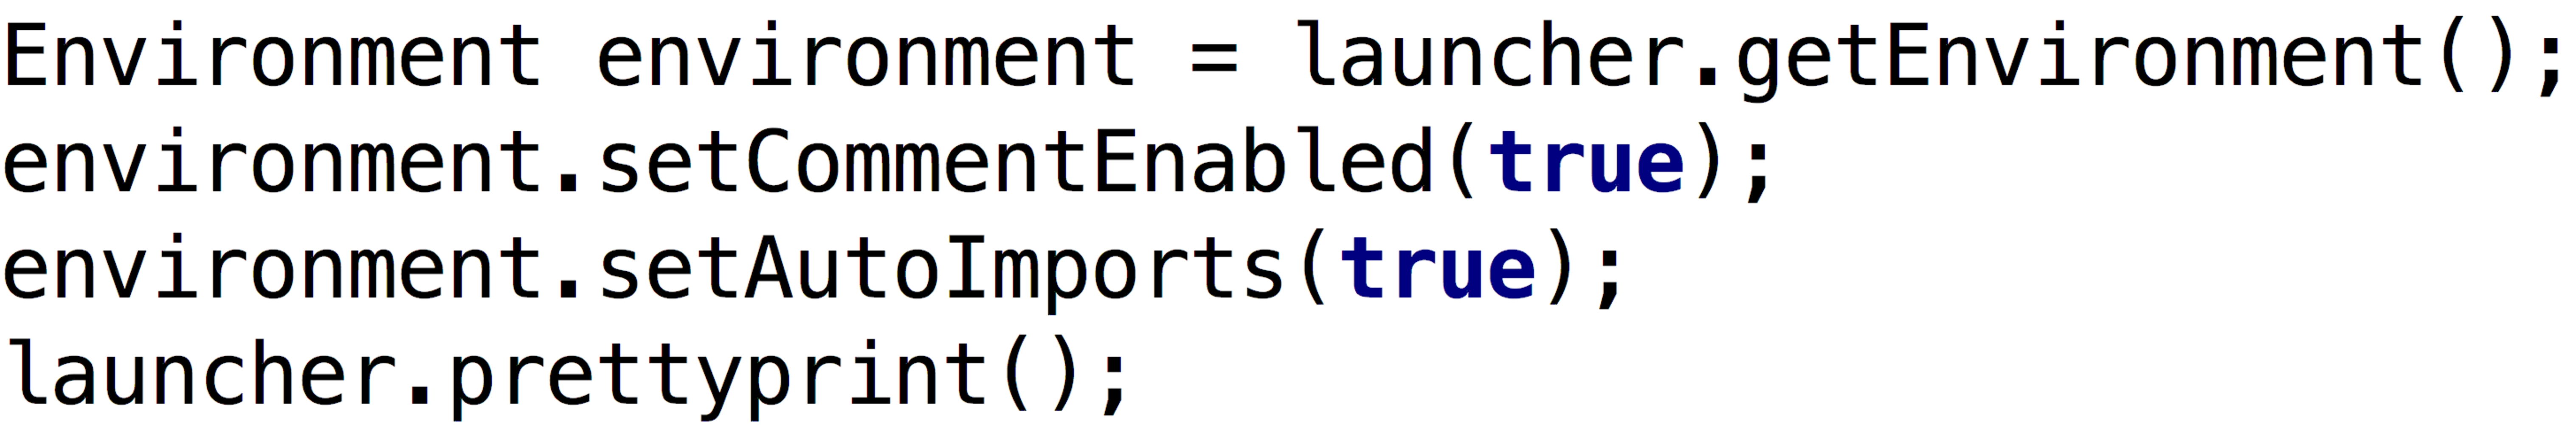
\includegraphics[width=\textwidth]{figures/output/prettyprint-imports-comments.pdf}
\end{figure}
\end{frame}

\begin{frame}{Output the model with imports and comments}

\begin{figure}
\centering
\includegraphics[width=\textwidth]{figures/output/scenario-result-2.pdf}
\end{figure}

\end{frame}

\begin{frame}{It looks tedious? Use Processors!}
Processors are a way to avoid calling all those steps: 

\begin{itemize}
\item A processor is created for a specific kind of node in Spoon Model
\item A process method is called each time the node type is encountered in the model
\item We can then check properties and/or transform the node or the model itself
\end{itemize}

Let's try it!
\end{frame}

\begin{frame}{Processor for our scenario - Structure}

\begin{figure}
\centering
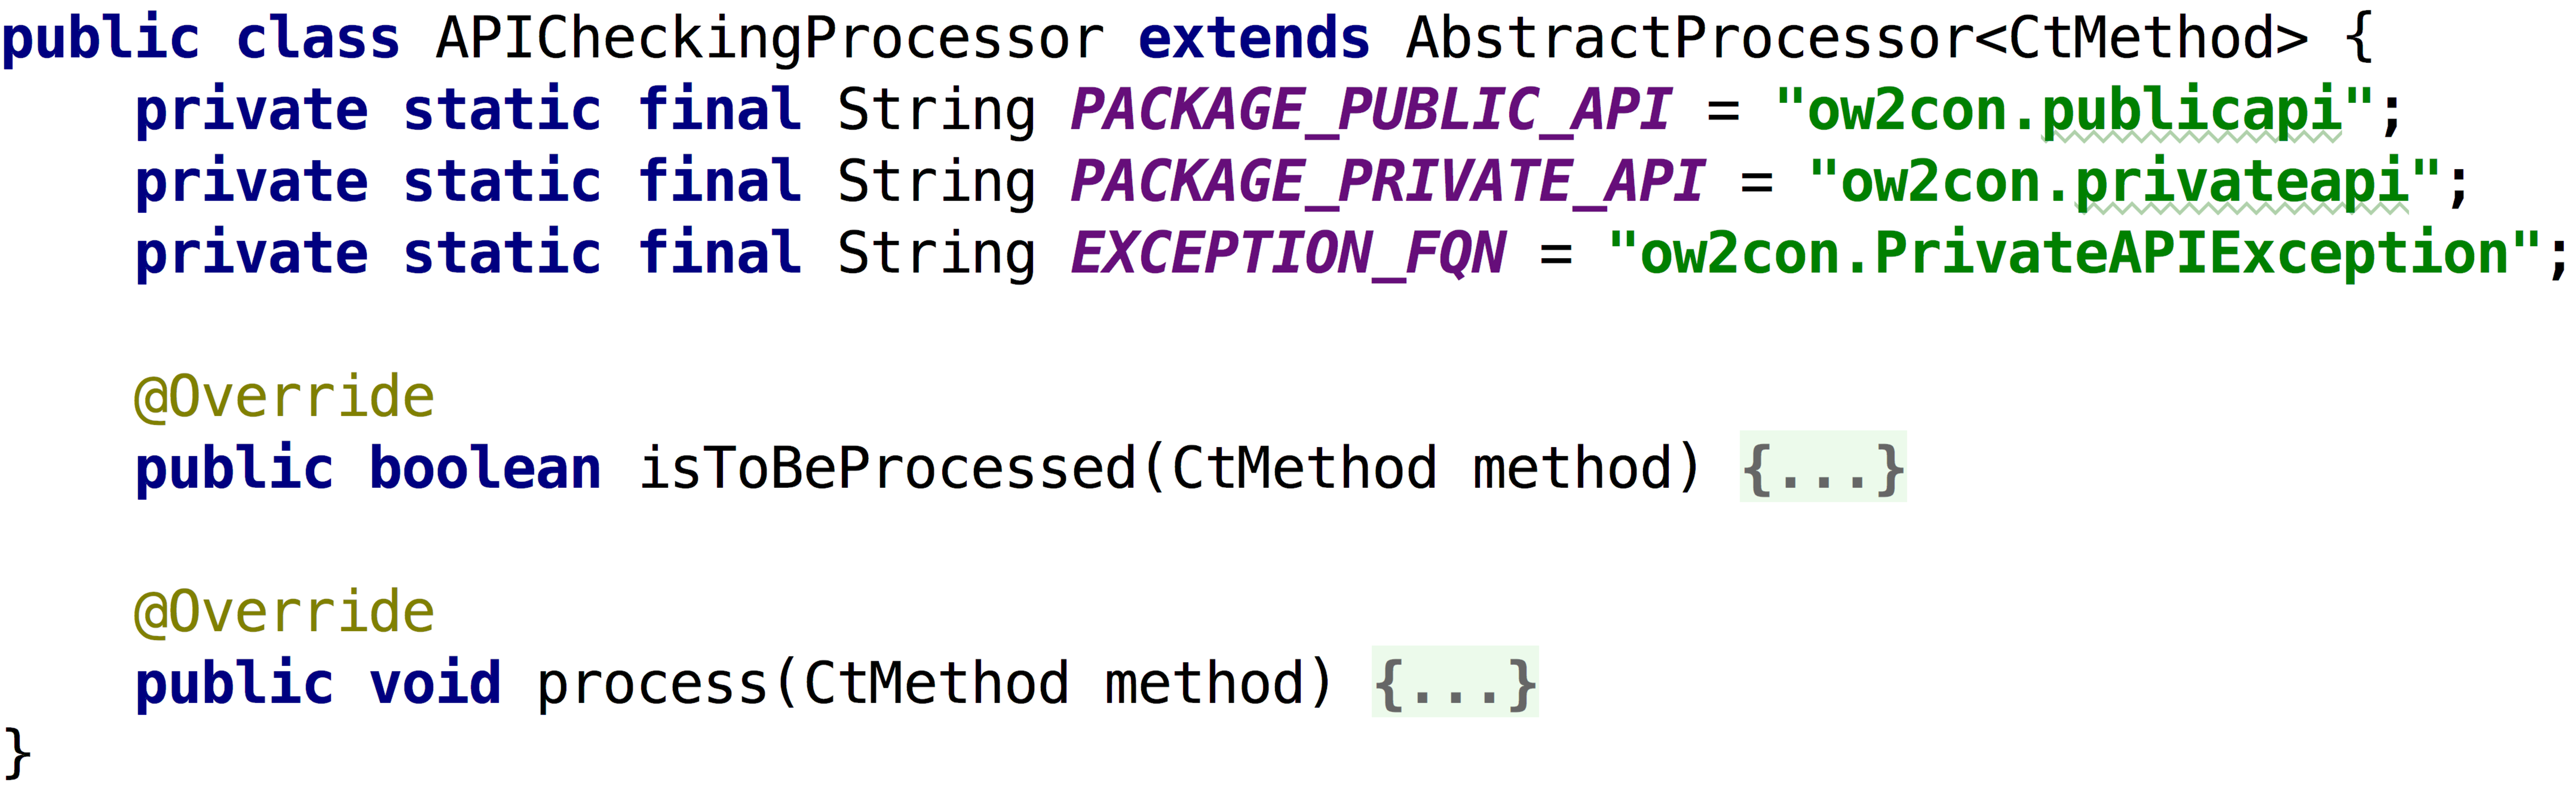
\includegraphics[width=\textwidth]{figures/processor/processor-structure.pdf}
\end{figure}
\end{frame}

\begin{frame}{Processor for our scenario - isToBeProcessed}

Method contains code to \textbf{query the model}
\begin{figure}
\centering
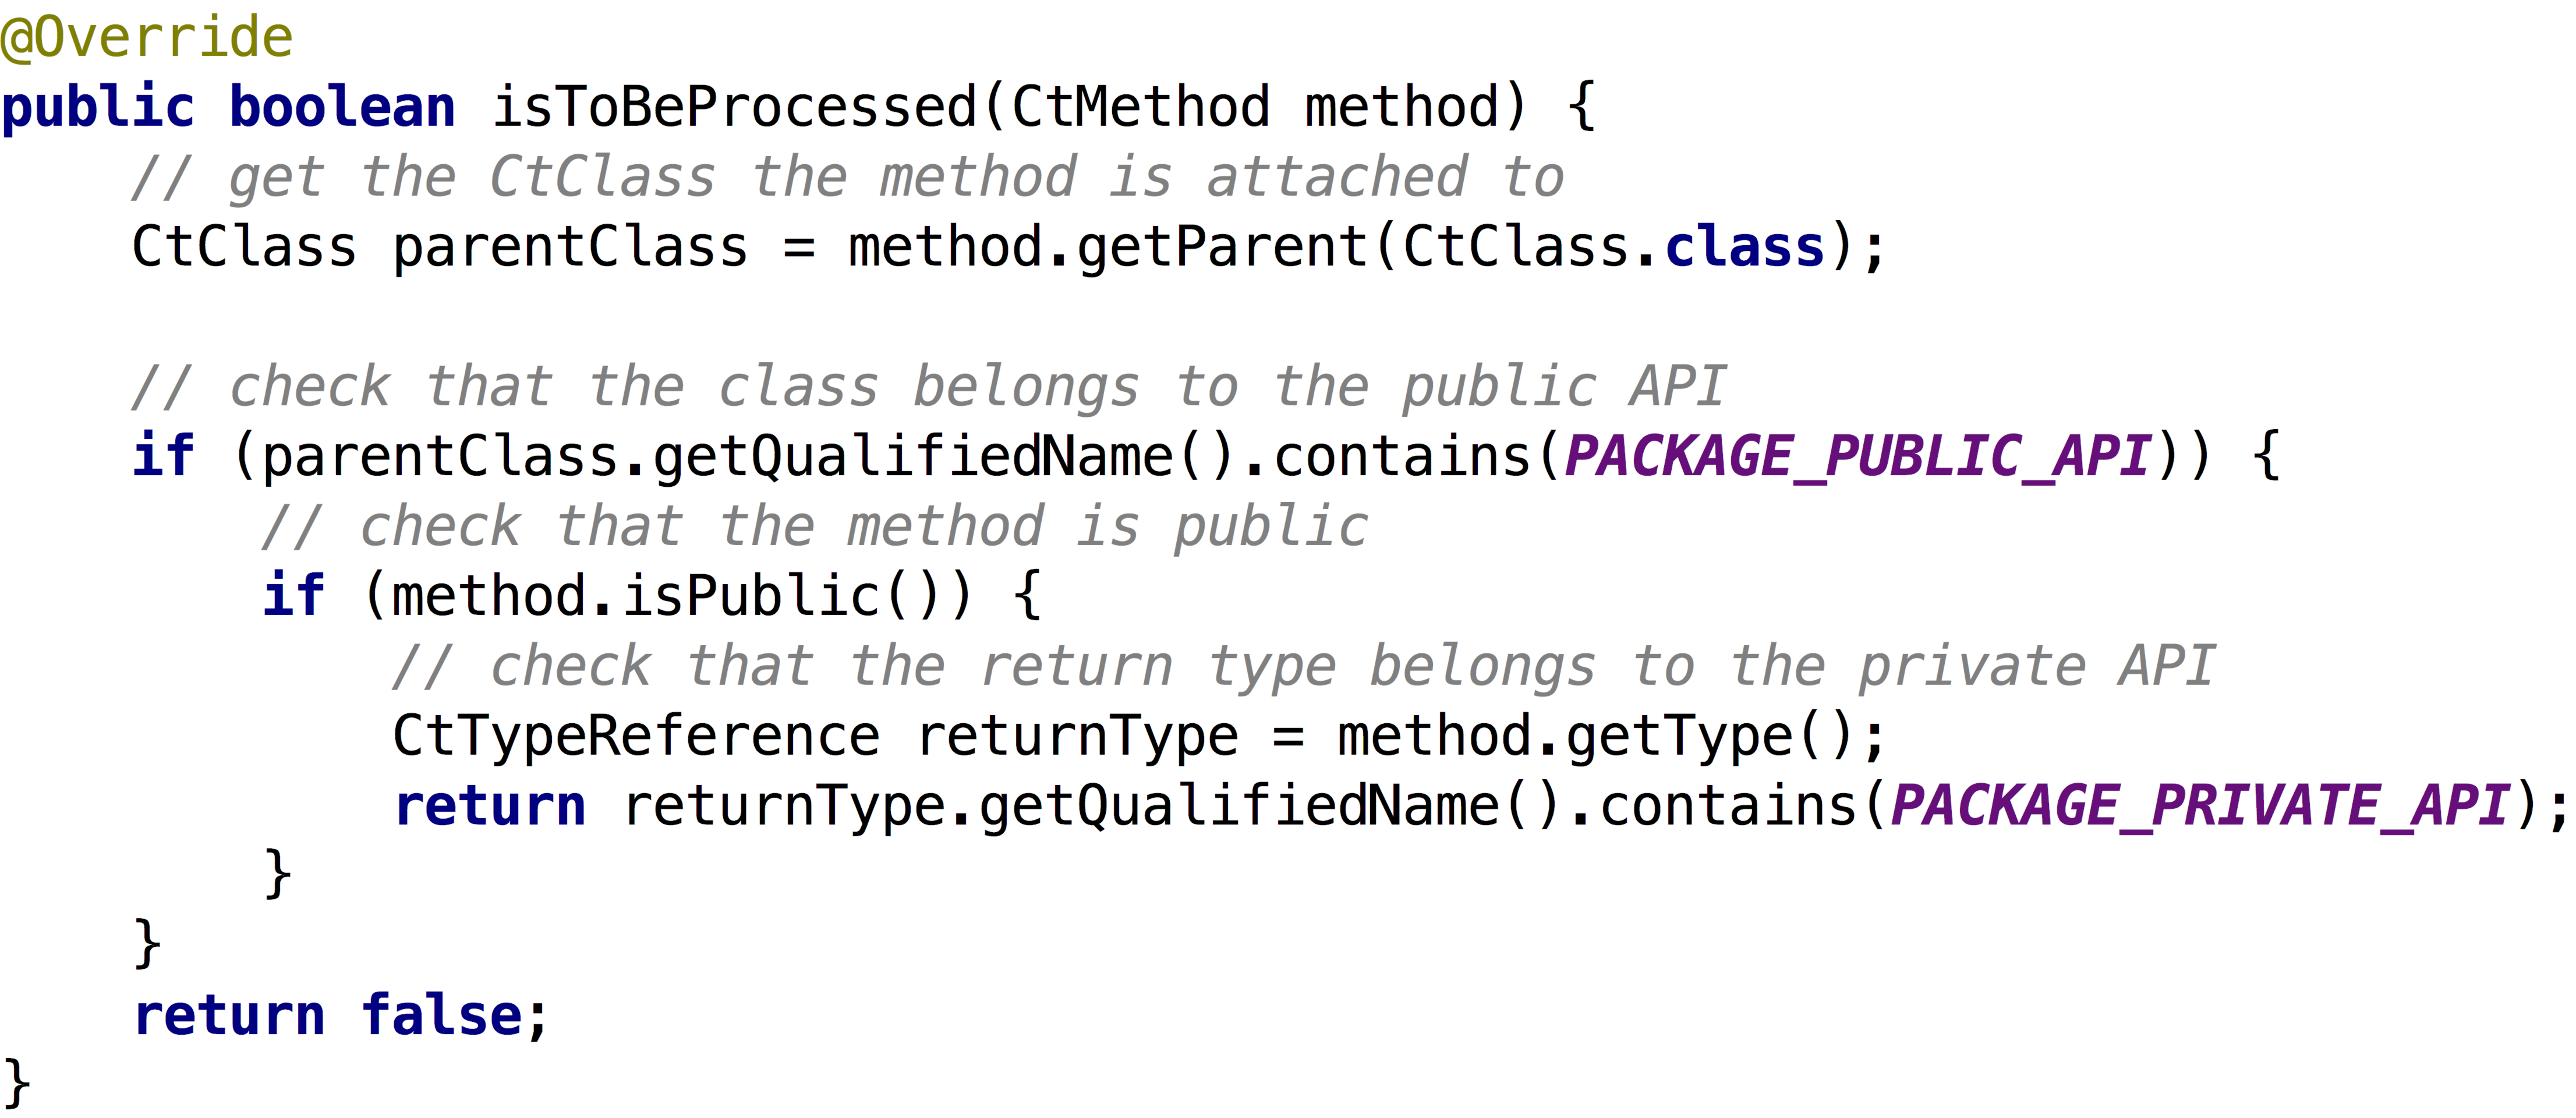
\includegraphics[width=\textwidth]{figures/processor/processor-is-to-be-processed.pdf}
\end{figure}
\end{frame}

\begin{frame}{Processor for our scenario - process}

Method contains code to \textbf{transform the model}
\begin{figure}
\centering
\includegraphics[width=\textwidth]{figures/processor/processor-process.pdf}
\end{figure}
\end{frame}

\begin{frame}{Processor usage from Java API}

\begin{figure}
\centering
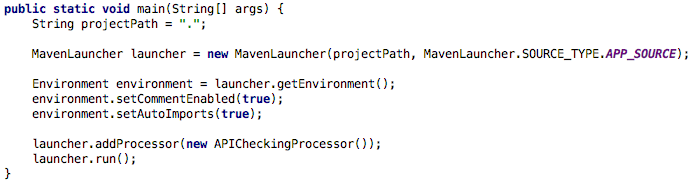
\includegraphics[width=\textwidth]{figures/processor/running-processor.png}
\end{figure}
\end{frame}

\begin{frame}{Processor usage from CLI}
\begin{figure}
\centering
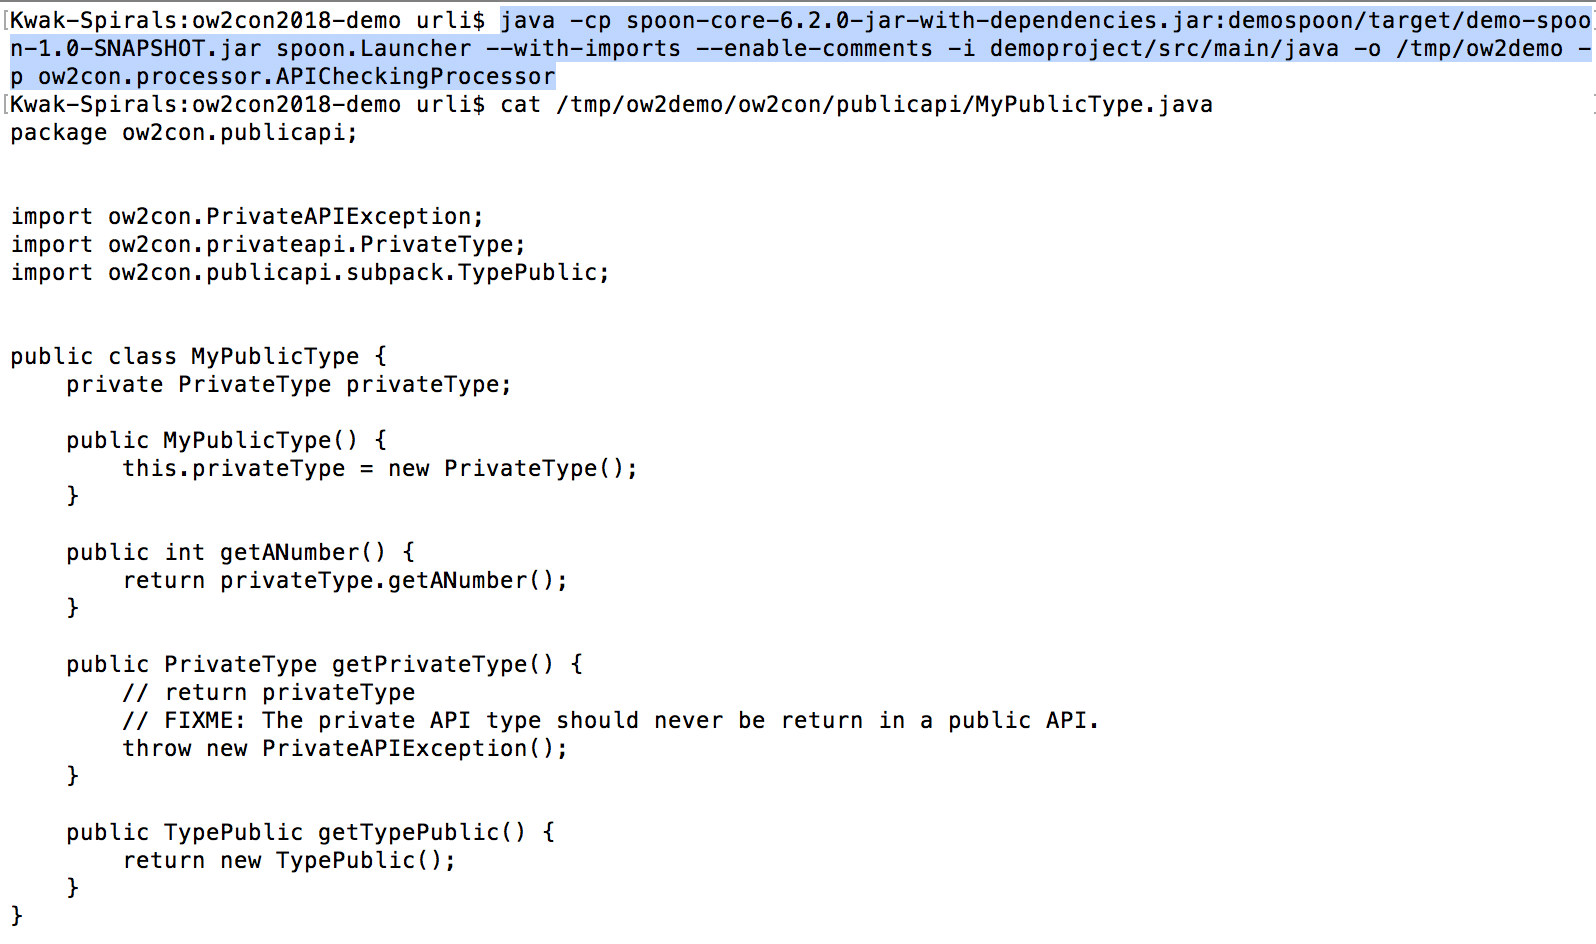
\includegraphics[width=\textwidth]{figures/processor/cli.png}
\end{figure}
\end{frame}

\begin{frame}{Processor usage from Maven Plugin}
\begin{figure}
\centering
\includegraphics[width=0.6\textwidth]{figures/processor/maven-config.pdf}
\end{figure}
\end{frame}

\begin{frame}{Conclusion}
Spoon is a multi-tool for Java Projects

This presentation was only about \textbf{a basic usage} of Spoon.

Projects are using Spoon for code analysis, program repair, code transpiling, or test amplification. 

Use it in your own projects: for architecture checking, code refactoring, test enforcing, ... 

New features are incoming to help you there!

We have an incredible community! 
Come help us improving Spoon API and get ready for Java 11 ;-)
\end{frame}

\end{document}
